\documentclass[uplatex,dvipdfmx,10pt,a4paper]{jsarticle}
\usepackage[margin=25mm]{geometry}
\usepackage[T1]{fontenc}
\usepackage{mathptmx}
\renewcommand{\ttdefault}{lmtt}
\usepackage[ipaex]{pxchfon}
\renewcommand{\headfont}{\mcfamily\bfseries}
\DeclareFontShape{JY2}{mc}{bx}{n}{<->ssub*mc/m/n}{}
\DeclareFontShape{JT2}{mc}{bx}{n}{<->ssub*mc/m/n}{}
\DeclareFontShape{JY2}{gt}{m}{n}{<->ssub*mc/m/n}{}
\DeclareFontShape{JT2}{gt}{m}{n}{<->ssub*mc/m/n}{}
\usepackage{url}
\usepackage{graphicx,booktabs,amsmath,url}
\renewcommand{\jsParagraphMark}{}
\usepackage[font=small,labelfont=bf]{caption}
\renewcommand{\figurename}{図}\renewcommand{\tablename}{表}
\title{\mcfamily\bfseries 生成ベース・トークン上限付き fitness による\\Qwen3.5-4B 派生 8 モデルの進化的線形マージ：\\Baphomet-1.1-4B\\[2pt]\large 技術報告書（ラウンド 2--3 を追加した改訂版）}
\author{CloudGoat}
\date{2026年11月}
\begin{document}
\maketitle

\begin{abstract}
Qwen3.5-4B を共通の基盤とする 8 つのファインチューンモデルについて，線形マージ係数を EvoGM 方式の進化的探索で求めた．fitness には，MMLU-Pro，GPQA，BFCL から取った 110 問に対し，チャットテンプレートと思考モードを有効にして\textbf{生成した}回答の素の正答率（上限 4,096 トークン）を用いた．第 1 ラウンド（40 候補，T4 GPU 7.1 時間）で得たマージは，fitness 用とは重複しない 180 問のテストで手動設定の均等マージ Baphomet-1.0-4B（$\lambda_i=0.1375$）と同等の正答率（77.2\% 対 77.8\%）を，半分の生成トークン数で達成した．続いて IRT で高速化した fitness を用いて探索をさらに 2 ラウンド続けた．40 問のサブセットをタスクごとの 2PL モデルで採点し，見込みの薄い候補は途中で打ち切り，有望な候補だけを 110 問で厳密に再評価する方式である（GPU 6.53 時間）．ラウンド 3 の勝者を \textbf{Baphomet-1.1-4B} として公開する．fitness は 0.764 で（ラウンド 1 勝者 0.722，最良の単体ドナー 0.686，Baphomet-1.0 0.603），180 問テストでも数値上は最高だった（79.4\%．Baphomet-1.0 は 77.8\%，基盤モデルは 70.0\%）．ただし Baphomet-1.0 に対する差は有意ではない（不一致ペア 10 対 7，McNemar $p=0.63$）．基盤モデルに対する差は有意である（20 対 3，$p<0.001$）．Baphomet-1.1 の生成トークン数は Baphomet-1.0 より 42\% 少ない（1,834 対 3,180）が，ラウンド 1 勝者（1,498）よりは多い．fitness は温度 0.6 の 1 サンプルであり，勝者はその fitness で選ばれ，テストも小さいため，これらは予備的な結果である．
\end{abstract}

\section{はじめに}
タスク算術によるマージでは，共通の基盤 $\theta_0$ に，各ファインチューンモデルのタスクベクトル $\tau_i=\theta_i-\theta_0$ を重み付きで足し合わせる．重み $\lambda_i$ は通常手で決める．Baphomet-1.0-4B はその一例で，Qwen3.5-4B 派生の 8 モデルを等しい重みで合成したものである．進化的探索を使えば $\lambda$ を自動で調整できるが，結果は fitness の設計に大きく左右される．以前の試み（MERGE$^3$ 方式，対数尤度による多肢選択の fitness，チャットテンプレートなし，MMLU-Pro と GPQA のみ）では，進化マージは生成回答で Baphomet に明確に負け，ツール呼び出しも劣化した．

本報告では，実際の使い方に近い fitness，すなわちチャットテンプレートと思考モードを有効にした生成回答を，ツール呼び出しのタスクを含めて，一定のトークン予算のもとで測るものを用いて再検討する．問いは二つである．(i) 進化で得た係数は均等マージを上回るか．(ii) 探索はどのようなマージを好むか．第\ref{sec:r1setup}--\ref{sec:r1res}節で第 1 ラウンドを，第\ref{sec:r2}--\ref{sec:r2res}節で IRT により高速化した fitness による追加の 2 ラウンドを述べる．その勝者を Baphomet-1.1-4B として公開する．

\section{実験設定}\label{sec:r1setup}
\paragraph{モデル．}基盤は Qwen/Qwen3.5-4B~\cite{qwen}．比較対象は均等マージの Baphomet-1.0-4B~\cite{baph}．本報告の最終モデル Baphomet-1.1-4B は EvoGM のラウンド 3 の勝者である（第\ref{sec:r2res}節）．ドナーは係数の順に Agents-A1，DeepSeek-V4-Pro 蒸留（\textit{dsv4pro}），Qwen3.8-Distill（\textit{q38distill}），Qwopus-Coder，Qwopus-v3，AREX-Turbo，NeoHorse，T-Max~\cite{m1,m2,m3,m4,m5,m6,m7,m8} で，いずれも同じ基盤から作られた 4B モデルである．ドナーに存在しないパラメータ（MTP ヘッド，ビジョン部など）の寄与は 0 とした．

\paragraph{マージ．}$\theta=\theta_0+\sum_{i=1}^{8}\lambda_i\tau_i$，$\lambda_i\in[-1,1]$，fp32 で累積．探索中のタスクベクトルは fp8 で保持した．Baphomet の再構成は公開重みと bf16 の 1 ulp 以内で一致した．マージ後の重みは常駐の vLLM エンジンにその場で読み込んだ．

\paragraph{探索．}EvoGM~\cite{evogm} の参照実装~\cite{evogmcode} を移植した（敗者を勝者へ写す 2 つの MLP 生成器を循環一貫性つきで学習．Adam，学習率 $10^{-4}$，反復ごとに 200 エポック，勝者は上位 30\%）．初期集団は 8 つの one-hot ベクトル，均等平均（$1/8$），Baphomet の係数からなる．EvoGM の探索は二重のループからなる．内側の反復（インナーループ）では，生成器を学習して新しい候補を作り，上位 $P$ 個を残す．外側のラウンド（アウターループ）は反復をまとめた単位で，終わりに上位 8 候補を新しい基底として入れ替える（basis shift）．本実験は集団サイズ $P=10$，ラウンド（アウターループ）1 回，ラウンドあたり反復（インナーループ）3 回，シード 42 で，評価した候補は計 40 である．ラウンドが 1 回のため，基底の入れ替えは行っていない（参照実装の既定は 2 ラウンド）．2$\times$T4 で GPU 10 時間の予算に収まるよう規模を決めた．

\paragraph{fitness．}110 問における 3 つの正答率の平均．内訳は MMLU-Pro 40 問，GPQA main/extended 30 問（Diamond は不使用），BFCL non-live 40 問（各カテゴリ 10 問）．生成はチャットテンプレートと思考モードを有効にし，温度 0.6，top-$p$ 0.95，top-$k$ 20，シード 0，上限 4,096 トークン．打ち切られた回答は不正解とした．IRT パラメータは情報量の多い問題を選ぶためだけに使い，採点には使っていない．

\paragraph{テスト．}fitness 用とは重複しない 180 問（MMLU-Pro 80，GPQA 50，BFCL 50）．生成設定は同じで，上限は 8,192 トークン．fitness 最大の勝者を，Baphomet および基盤モデルと同一の問題で比較した．有意性は不一致ペアに対する正確な両側 McNemar 検定（符号検定）で評価した．

\section{ラウンド 1 の結果}\label{sec:r1res}
\paragraph{探索．}推移を図\ref{fig:traj}に示す．初期集団で最良だったのはドナー q38distill 単体（0.686）で，Baphomet は 0.603，均等平均は 0.592 だった（表\ref{tab:init}）．最良 fitness は反復 1 で 0.697，反復 2 で 0.722 に上がり，反復 3 では改善しなかった．評価に失敗した候補はなかった．

\begin{figure}[htbp]
\centering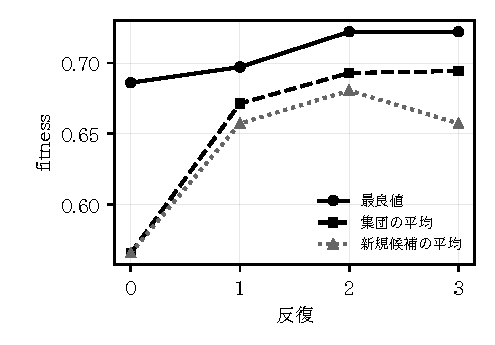
\includegraphics[width=0.55\textwidth]{fig_traj_ja.pdf}
\caption{ラウンド 1：反復ごとの fitness（110 問，上限 4,096 トークン）．}
\label{fig:traj}
\end{figure}

\begin{table}[htbp]
\centering\small
\caption{fitness 用問題における初期集団．トークン＝平均生成トークン数．}
\label{tab:init}
\setlength{\tabcolsep}{3.5pt}
\begin{tabular}{lcccrr}
\toprule
候補 & MMLU & GPQA & BFCL & fitness & トークン \\
\midrule
q38distill & .70 & .43 & .93 & .686 & 671 \\
dsv4pro & .68 & .47 & .85 & .664 & 1,331 \\
Qwopus-v3 & .70 & .23 & .93 & .619 & 1,835 \\
Baphomet & .65 & .23 & .93 & .603 & 1,925 \\
均等平均（$1/8$） & .68 & .20 & .90 & .592 & 2,073 \\
Qwopus-Coder & .65 & .17 & .88 & .564 & 1,834 \\
NeoHorse & .60 & .03 & .90 & .511 & 2,180 \\
T-Max & .50 & .13 & .90 & .511 & 2,343 \\
AREX-Turbo & .42 & .07 & .95 & .481 & 1,924 \\
Agents-A1 & .45 & .07 & .75 & .422 & 2,492 \\
\midrule
\textbf{ラウンド 1 勝者} & .80 & .47 & .90 & \textbf{.722} & 1,096 \\
\bottomrule
\end{tabular}
\end{table}

\paragraph{勝者の係数．}ラウンド 1 勝者の係数は次のとおりである．\begin{align*}\lambda^\star = (&0.007,\ 0.104,\ 0.627,\ 0.015,\ 0.233,\ 0.053,\ -0.004,\ 0.010)\end{align*}重みの大半は q38distill（0.63）と Qwopus-v3（0.23）にあり，dsv4pro に少し（0.10），それ以外はほぼ 0 である（$\sum\lambda_i=1.05$．Baphomet は 1.10）．上位の他の候補も，単体で最も強い 3 モデル（dsv4pro，q38distill，Qwopus-v3）を主に混ぜていた．

\paragraph{テスト．}180 問の結果は表\ref{tab:test}（第\ref{sec:r2res}節）に示す．全体の正答率でラウンド 1 勝者と Baphomet-1.0 に統計的な差はない（勝ち 8 問，負け 9 問，$p=1.0$）．スイート別では GPQA で 4.0 ポイント上回り，MMLU-Pro（$-2.5$）と BFCL（$-2.0$）で下回ったが，いずれも有意ではない．基盤モデルに対しては勝ち 18 問，負け 5 問（$p=0.011$）で，主に GPQA（12 対 2，$p=0.013$）による．

\paragraph{推論の長さ．}ラウンド 1 勝者の生成トークン数は Baphomet より全体で 53\%，MMLU-Pro で 64\%，GPQA で 45\% 少なく，打ち切り率は半分以下だった．40 候補全体で fitness と平均生成長には強い負の相関がある（Spearman $\rho=-0.65$，$p<10^{-5}$．図\ref{fig:scatter}）．

\begin{figure}[htbp]
\centering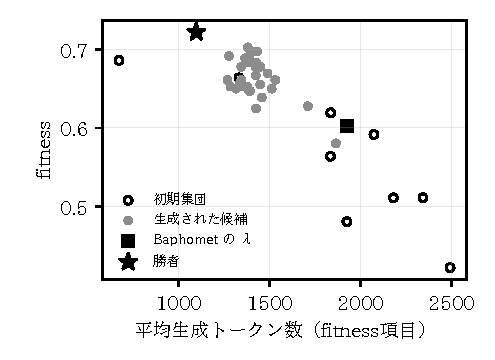
\includegraphics[width=0.55\textwidth]{fig_scatter_ja.pdf}
\caption{ラウンド 1：全 40 候補の fitness と平均生成トークン数．}
\label{fig:scatter}
\end{figure}

\section{ラウンド 2--3：IRT による高速化探索}\label{sec:r2}
第 1 ラウンドでは全候補を 110 問の fitness で評価しており（1 候補あたり生成だけで約 1,000 秒），EvoGM の外側ループに回す予算が残らなかった．そこで追加の上限 GPU 8 時間のもとで探索を続けるため，保存した探索状態から再開し，全問評価の大半を安価な推定値に置き換えた．

\paragraph{IRT サブセットと推定量．}ラウンド 1 の 40 候補 $\times$ 110 問の正誤行列（打ち切り＝不正解）に，タスク（MMLU-Pro，GPQA，BFCL）ごとの 2PL 項目反応モデルを同時 MAP 推定で当てはめた（$\theta\sim\mathcal N(0,1)$，$\log a\sim\mathcal N(0,0.5^2)$，$b\sim\mathcal N(0,2^2)$）．タスクごとに，上位 15 候補の能力値における Fisher 情報量を $\sqrt{\text{平均トークン数}}$ で割った値が大きい問題を残した．MMLU-Pro 16 問，GPQA 10 問，BFCL 14 問の計 40 問である（1 候補あたり約 6.6 万トークン．全問では約 16.5 万）．新しい候補はこの 40 問だけに回答する．タスクごとの fitness 推定値は，サブセットでの正答数に，未観測の問題に対する 2PL 確率 $p(\theta_{\text{MAP}})$ の和を足し，タスクの問題数で割ったものである．3 タスクの値を平均するので，推定値はラウンド 1 の fitness と同じ尺度になる．ラウンド 1 の 40 候補での一個抜き検証では，全問 fitness に対する平均絶対誤差（MAE）が 0.013（上位 15 候補では 0.009），順位相関が 0.93 だった．サブセットの単純な正答率では MAE 0.066 である．

\paragraph{レーシング．}生成中の出力を逐次受け取り，サブセットの半分以上が終わった時点で楽観的な推定値（$\theta+1.5\,\text{sd}$）を計算する．これが現在の集団の $P$ 番目の値を下回れば，その候補の生成を打ち切る．ラウンド 1 の反復 2--3 を使ったオフラインのシミュレーションでは，20 候補中 4 候補を打ち切り，時間を約 9\% 節約し，誤って打ち切った候補はなかった．

\paragraph{完全評価のルール．}推定誤差と勝者の呪いに備え，各反復の後に，まだ完全評価していない集団メンバーのうち最良のものの推定値が，それまでの最良の厳密 fitness から 0.02 以内であれば，上位 2 メンバーを残り 70 問で評価した（GPU 1 枚に 1 候補）．これでラウンド 1 と同じ定義の厳密な 110 問 fitness が得られる．集団と生成器には，得られている最良の値（厳密値があればそれ，なければ推定値）を使う．最終的な勝者は，ラウンド 1 と全ての完全評価を通じて\textbf{厳密な} 110 問 fitness が最大の候補であり，180 問テストはその候補だけで行う．

\paragraph{探索の進め方．}各ラウンドの最初に基底を入れ替える．前ラウンドまでの履歴の上位 8 候補が新しいエキスパートとなり（ラウンド 2 では fitness .722，.703，.697，.697，.692，.692，.689，.686），探索はその座標系で行う．$P=10$，生成器はラウンドごとに初期化し，ラウンドあたり最大 3 反復とした．ラウンドと反復の数は，計測したコストからカーネル内で決め，最終テストの時間は常に確保した．

\section{ラウンド 2--3：結果}\label{sec:r2res}
\paragraph{実行．}実行は 2$\times$T4 で GPU 6.53 時間（上限 8 時間）で終わった．ラウンド 2 と 3 をそれぞれ 3 反復で完了し，ラウンド 4 は残り 0.88 時間が 1 ラウンドの最低所要 0.92 時間に満たないため省略した．新規のサブセット評価は 64 回（ラウンド 1 と合わせて計 104 候補），完全評価は 12 回で，レーシングで途中打ち切りになった候補は 3，失敗した候補は 0 だった．

\paragraph{探索の推移．}最良の厳密 fitness はラウンド 2 の間はラウンド 1 の値 0.722 のままで（完全評価した候補の 1 つが同点），ラウンド 3 の反復 2 で 0.733，反復 3 で 0.764 に上がった（図\ref{fig:search}左）．完全評価した 12 候補では，IRT 推定値と厳密 fitness の MAE は 0.009，Spearman 相関は 0.96，平均バイアスは $+0.008$ だった（図\ref{fig:search}右）．推定値が高いものを選んで完全評価しているので，このバイアスは想定どおりである．最も顕著なのは勝者で，推定値 0.782 に対し厳密 fitness は 0.764 だった．

\begin{figure}[htbp]
\centering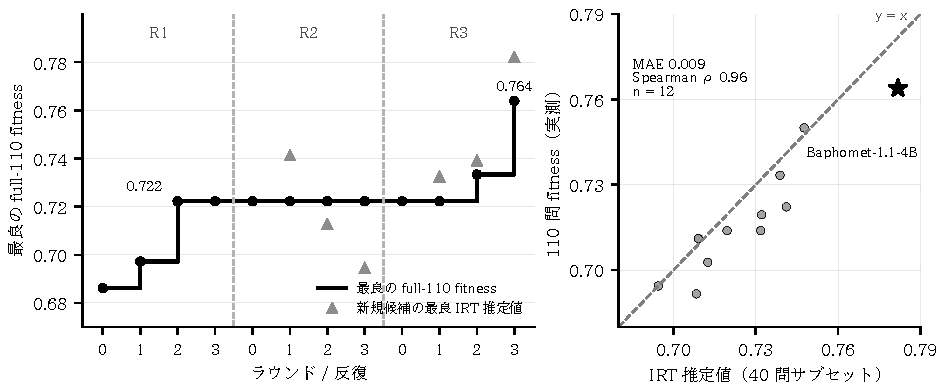
\includegraphics[width=\textwidth]{fig_search_r2_ja.pdf}
\caption{左：ラウンド 1--3 の各反復後の，その時点までの最良の厳密 110 問 fitness（反復 0＝そのラウンドの初期集団）．三角は各反復の新規候補のうち最良の IRT 推定値（ラウンド 2--3）．右：完全評価した 12 候補の IRT 推定値と厳密 110 問 fitness．星が Baphomet-1.1-4B．}
\label{fig:search}
\end{figure}

\paragraph{Baphomet-1.1-4B の係数．}ラウンド 3 の勝者の係数は
\begin{align*}\lambda_{1.1} = (&0.0116,\ 0.2039,\ 0.5901,\ 0.0013,\ 0.2972,\ 0.0323,\ 0.0030,\ -0.0007)\end{align*}
で（順に Agents-A1，dsv4pro，q38distill，Qwopus-Coder，Qwopus-v3，AREX-Turbo，NeoHorse，T-Max），$\sum\lambda_i=1.14$ である．ラウンド 1 勝者と同じ 3 ドナーを使いつつ，q38distill（0.63\,$\to$\,0.59）から dsv4pro（0.10\,$\to$\,0.20）と Qwopus-v3（0.23\,$\to$\,0.30）へ重みを移している．残り 5 ドナーはほぼ 0 のままである（図\ref{fig:lambda}）．

\begin{figure}[htbp]
\centering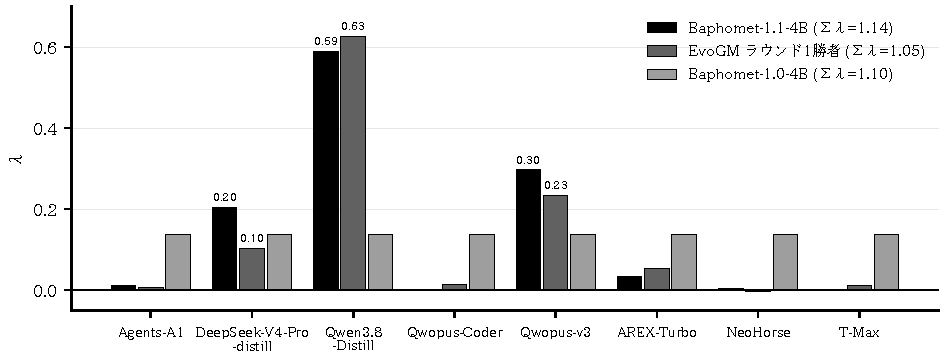
\includegraphics[width=\textwidth]{fig_lambda_ja.pdf}
\caption{Baphomet-1.1-4B，ラウンド 1 勝者，Baphomet-1.0-4B のマージ係数．}
\label{fig:lambda}
\end{figure}

\paragraph{fitness セットでのエキスパートとの比較．}表\ref{tab:fit110}と図\ref{fig:fit110}--\ref{fig:fit110eff}に，110 問の fitness 用問題（上限 4,096 トークン）での Baphomet-1.1，8 つのドナー，均等平均，Baphomet-1.0，ラウンド 1 勝者の比較を示す．Baphomet-1.1 の fitness が最も高く（0.764），最良の単体ドナー（q38distill，0.686）を 0.078，Baphomet-1.0（0.603）を 0.161 上回る．MMLU-Pro（.800）と GPQA（.567）では 1 位または同率 1 位だが，BFCL では AREX-Turbo の方が高い（.950 対 .925）．注意点が二つある．Baphomet-1.1 はこの問題で\textbf{選ばれた}モデルなので，そのスコアは楽観的に偏っている（ドナーのスコアにはこの偏りはない）．また，ドナーはこのセットでのみ評価しており，180 問テストでは\textbf{評価していない}．

\begin{table}[htbp]
\centering\small
\caption{110 問 fitness セット（上限 4,096 トークン）．fitness＝3 タスクの正答率の平均，打切＝打ち切られた回答の割合（\%），トークン＝平均生成トークン数．Baphomet-1.1 とラウンド 1 勝者はこの問題で選ばれた（楽観的）．ドナーは 180 問テストでは未評価．}
\label{tab:fit110}
\setlength{\tabcolsep}{3.5pt}
\begin{tabular}{lcccrrr}
\toprule
モデル & MMLU & GPQA & BFCL & fitness & 打切 & トークン \\
\midrule
\textbf{Baphomet-1.1-4B} & .800 & .567 & .925 & \textbf{.764} & 11.8 & 1,149 \\
ラウンド 1 勝者 & .800 & .467 & .900 & .722 & 12.7 & 1,096 \\
\midrule
q38distill & .700 & .433 & .925 & .686 & 3.6 & 671 \\
dsv4pro & .675 & .467 & .850 & .664 & 19.1 & 1,331 \\
Qwopus-v3 & .700 & .233 & .925 & .619 & 27.3 & 1,835 \\
Qwopus-Coder & .650 & .167 & .875 & .564 & 33.6 & 1,834 \\
NeoHorse & .600 & .033 & .900 & .511 & 40.0 & 2,180 \\
T-Max & .500 & .133 & .900 & .511 & 41.8 & 2,343 \\
AREX-Turbo & .425 & .067 & .950 & .481 & 28.2 & 1,924 \\
Agents-A1 & .450 & .067 & .750 & .422 & 48.2 & 2,492 \\
\midrule
Baphomet-1.0-4B & .650 & .233 & .925 & .603 & 31.8 & 1,925 \\
均等平均（$1/8$） & .675 & .200 & .900 & .592 & 30.9 & 2,073 \\
\bottomrule
\end{tabular}
\end{table}

\begin{figure}[htbp]
\centering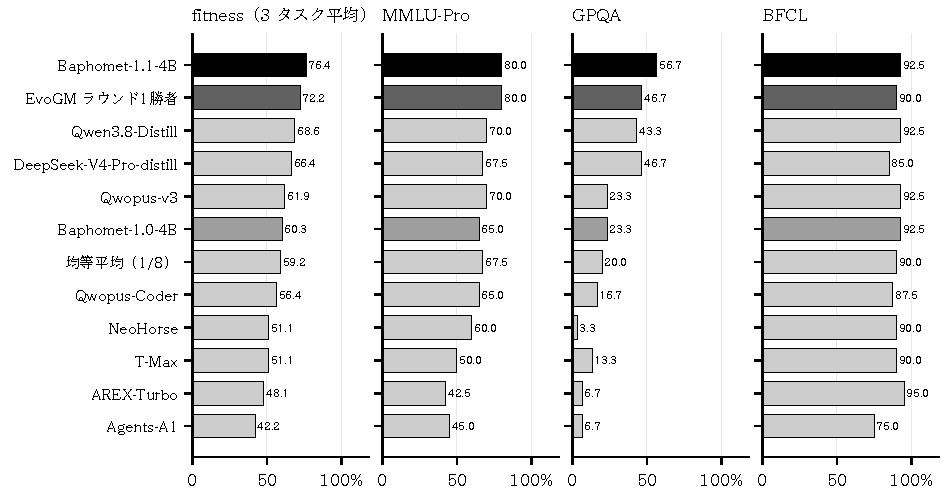
\includegraphics[width=\textwidth]{fig_fit110_acc_ja.pdf}
\caption{110 問 fitness セットにおける fitness とタスク別正答率（Baphomet-1.1-4B，ラウンド 1 勝者，8 ドナー，Baphomet-1.0-4B，均等平均）．Baphomet-1.1 はこの問題で選ばれたため，そのスコアは楽観的である．}
\label{fig:fit110}
\end{figure}

\begin{figure}[htbp]
\centering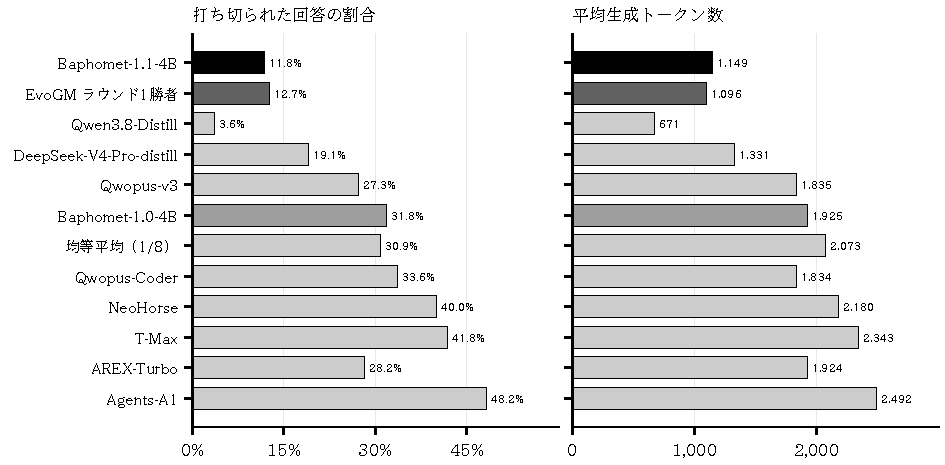
\includegraphics[width=\textwidth]{fig_fit110_eff_ja.pdf}
\caption{110 問 fitness セットにおける打ち切り率と平均生成トークン数（モデルと順序は図\ref{fig:fit110}と同じ）．}
\label{fig:fit110eff}
\end{figure}

\paragraph{テスト．}テストで評価した 4 モデルの 180 問の結果を表\ref{tab:test}と図\ref{fig:test}に示す（ドナーと均等平均は未評価）．Baphomet-1.1 は全体で数値上最も高く（79.4\%，Wilson 95\% 信頼区間 73.0--84.7），Baphomet-1.0（77.8\%，71.2--83.2），ラウンド 1 勝者（77.2\%，70.6--82.7），Qwen3.5-4B（70.0\%，62.9--76.2）が続く．信頼区間は大きく重なっている．対応のある検定（表\ref{tab:mcnemar}）では，Baphomet-1.1 は Baphomet-1.0（勝ち 10 問，負け 7 問，$p=0.63$）にもラウンド 1 勝者（12 対 8，$p=0.50$）にも\textbf{有意には}勝っていない．基盤モデルには有意に勝っており（20 対 3，$p<0.001$），主に GPQA（10 対 0，$p=0.002$）と MMLU-Pro（9 対 1，$p=0.021$）による．Baphomet-1.0 に対するスイート別の差は MMLU-Pro で +3.8 ポイント，GPQA で +4.0，BFCL で $-4.0$（不一致ペア 0 対 2）で，いずれも有意ではない．

\begin{table}[htbp]
\centering\small
\caption{180 問テスト（上限 8,192 トークン）．正答率は\%，打切＝打ち切られた回答の割合（\%），トークン＝平均生成トークン数．ドナーはこのテストでは未評価．}
\label{tab:test}
\setlength{\tabcolsep}{4pt}
\begin{tabular}{llrrr}
\toprule
スイート（$n$） & モデル & 正答率 & 打切 & トークン \\
\midrule
MMLU-Pro（80） & \textbf{Baphomet-1.1-4B} & \textbf{81.3} & 5.0 & 1,492 \\
 & ラウンド 1 勝者 & 75.0 & 5.0 & 1,200 \\
 & Baphomet-1.0-4B & 77.5 & 13.8 & 3,331 \\
 & Qwen3.5-4B & 71.3 & 17.5 & 4,385 \\
\midrule
GPQA（50） & \textbf{Baphomet-1.1-4B} & \textbf{62.0} & 28.0 & 4,007 \\
 & ラウンド 1 勝者 & 62.0 & 16.0 & 3,270 \\
 & Baphomet-1.0-4B & 58.0 & 34.0 & 5,915 \\
 & Qwen3.5-4B & 42.0 & 54.0 & 7,094 \\
\midrule
BFCL（50） & \textbf{Baphomet-1.1-4B} & 94.0 & 0.0 & 207 \\
 & ラウンド 1 勝者 & 96.0 & 0.0 & 202 \\
 & Baphomet-1.0-4B & \textbf{98.0} & 0.0 & 205 \\
 & Qwen3.5-4B & 96.0 & 0.0 & 229 \\
\midrule
全体（180） & \textbf{Baphomet-1.1-4B} & \textbf{79.4} & 10.0 & 1,834 \\
 & ラウンド 1 勝者 & 77.2 & 6.7 & 1,498 \\
 & Baphomet-1.0-4B & 77.8 & 15.6 & 3,180 \\
 & Qwen3.5-4B & 70.0 & 22.8 & 3,983 \\
\bottomrule
\end{tabular}
\end{table}

\begin{table}[htbp]
\centering\small
\caption{180 問テストでの対応のある比較．前者だけが正解した問題数--後者だけが正解した問題数と，正確な両側 McNemar 検定の $p$ 値．}
\label{tab:mcnemar}
\setlength{\tabcolsep}{4pt}
\begin{tabular}{lcccc}
\toprule
比較 & 全体 & MMLU-Pro & GPQA & BFCL \\
\midrule
Baphomet-1.1 対 Baphomet-1.0 & 10--7（$p$=.63） & 5--2（.45） & 5--3（.73） & 0--2（.50） \\
Baphomet-1.1 対 ラウンド 1 勝者 & 12--8（.50） & 7--2（.18） & 5--5（1.0） & 0--1（1.0） \\
Baphomet-1.1 対 Qwen3.5-4B & 20--3（$<$.001） & 9--1（.021） & 10--0（.002） & 1--2（1.0） \\
ラウンド 1 勝者 対 Baphomet-1.0 & 8--9（1.0） & 3--5（.73） & 5--3（.73） & 0--1（1.0） \\
Baphomet-1.0 対 Qwen3.5-4B & 17--3（.003） & 7--2（.18） & 9--1（.021） & 1--0（1.0） \\
\bottomrule
\end{tabular}
\end{table}

\begin{figure}[htbp]
\centering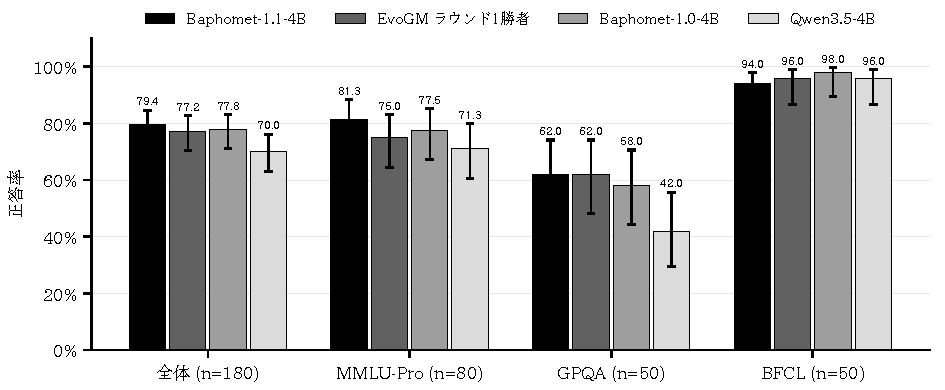
\includegraphics[width=\textwidth]{fig_test180_acc_ja.pdf}
\caption{180 問テストの正答率と Wilson 95\% 信頼区間（上限 8,192 トークン）．テストで評価したのはこの 4 モデルのみで，8 ドナーと均等平均は未評価．}
\label{fig:test}
\end{figure}

\paragraph{推論の長さ．}Baphomet-1.1 の生成トークン数は Baphomet-1.0 より全体で 42\% 少なく（1,834 対 3,180．MMLU-Pro で 55\%，GPQA で 32\% 少ない），打ち切りも少ない（10.0\% 対 15.6\%）．一方，ラウンド 1 勝者と比べると長く（1,834 対 1,498 トークン），打ち切りも多い（10.0\% 対 6.7\%）．その差はほぼ GPQA によるものである（打ち切り 28\% 対 16\%．図\ref{fig:testeff}）．ラウンド 1 勝者に対する正答率の上積みの一部は，推論が長くなったことと引き換えに得られている．

\begin{figure}[htbp]
\centering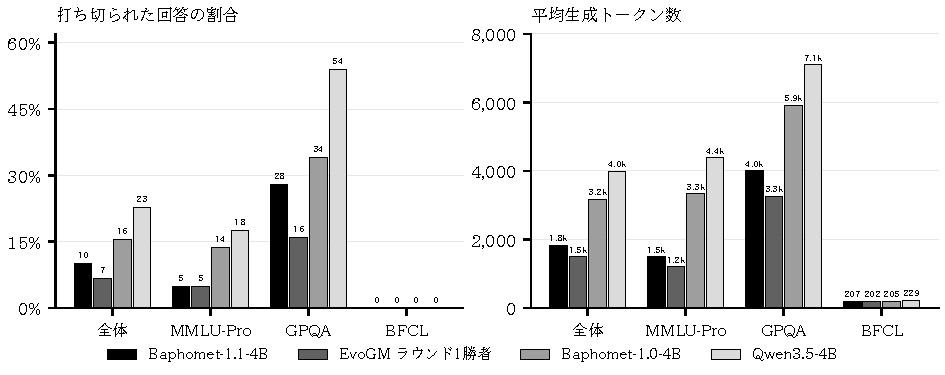
\includegraphics[width=\textwidth]{fig_test180_eff_ja.pdf}
\caption{180 問テストにおける打ち切り率と平均生成トークン数．}
\label{fig:testeff}
\end{figure}

\section{考察}
\paragraph{追加ラウンドで得たもの．}2 ラウンドの追加で，最良の厳密 fitness は 0.722 から 0.764 に，テスト正答率は 77.2\% から 79.4\% に上がった．ただしラウンド 1 勝者に対するテストでの差（不一致ペア 12 対 8）も，Baphomet-1.0 に対する差（10 対 7）も有意ではない．Baphomet-1.1 は我々が測ったなかで数値上最良のモデルであって，Baphomet-1.0 より良いことが示されたわけではない．

\paragraph{勝者の呪い．}勝者は多数のノイズを含む測定値の最大値なので，測定値は真の性能を過大に見積もる．本実験ではこれが二重に起きている．第一に，IRT 推定値が高いために完全評価に選ばれた勝者は，推定値が厳密 fitness を上回っていた（0.782 対 0.764）．完全評価した候補全体でも平均 $+0.008$ の偏りがある．第二に，厳密な 110 問 fitness 自体も小さな問題セットに対する温度 0.6 の 1 サンプルであり，勝者は 52 個の厳密値（ラウンド 1 の 40 候補と，64 の新規候補から選んだ 12 の完全評価）の最大値である．このセットでのラウンド 1 勝者に対する 0.042 のリードの一部は，選択によるノイズである可能性が高い．選択に一切使っていない 180 問テストが偏りのない比較であり，そこでのリードは 2.2 ポイントに縮む．

\paragraph{効率．}ラウンド 1 の結果は，上限付きの生成 fitness が短い推論を選ぶことを示唆していた．ラウンド 2--3 で得たマージは，ラウンド 1 勝者より正確だがやや長い（テストで 1,834 対 1,498 トークン，GPQA の打ち切り 28\% 対 16\%）．それでも Baphomet-1.0 よりは明らかに短い．fitness の上限 4,096 トークンでは両勝者の長さはほぼ同じ（1,149 対 1,096 トークン）なので，差は主にテストの大きな上限で現れている．

\paragraph{IRT による高速化．}40 問の推定量は，全問評価の約 40\% のトークンで探索を導くのに十分な精度だった（完全評価した候補で MAE 0.009，順位相関 0.96）．完全評価のルールにより最終的な選択は厳密値で行ったので，残る IRT の偏りはどの候補を完全評価するかには影響するが，報告した勝者の fitness には影響しない．

\paragraph{fitness 設計の影響．}以前の対数尤度による探索では，得られたマージが Baphomet に負け（90 問の部分集合で不一致ペア 2 対 17），ツール呼び出しも壊れた．ツール使用タスクを含む生成ベースの fitness では，ツール呼び出しを保ち（BFCL 94--96\%），Baphomet-1.0 と同等以上のマージが得られた．ただし両実験は fitness 以外（マージ手法，ドナー数，探索アルゴリズム）も異なるため，この比較は示唆にとどまる．

\section{限界}
探索は 1 回・シード 1 つのみである．110 問 fitness は温度 0.6 の 1 サンプルで，勝者はそれで選ばれているため，fitness セットでのドナーとの比較は Baphomet-1.1 に有利に偏っている．完全評価していない候補（レーシングで打ち切った 3 候補を含む）は IRT 推定値しかない．180 問テストは小さく，2--4 ポイントの差は有意にならない．ドナーと均等平均はテストで評価していない．fitness はテストより短いトークン上限で測っており，どのモデルでも誤答の一部は打ち切りによるので，上限を大きくすれば正答率は変わりうる．ドナーの説明は各モデルカードに従っており，独自には検証していない．

\section{結論}
生成ベース・トークン上限付きの fitness を用いた EvoGM 方式の探索を，IRT で高速化した推定量によりさらに 2 ラウンド（GPU 6.53 時間）続け，Baphomet-1.1-4B を得た．fitness セットでは最良であり（0.764．最良のドナーは 0.686，Baphomet-1.0 は 0.603．ただし選択の偏りは 1.1 に有利），重複のない 180 問テストでも数値上最良だった（79.4\%．Baphomet-1.0 は 77.8\%，Qwen3.5-4B は 70.0\%）．しかし Baphomet-1.0 より有意に良いとは言えない（$p=0.63$）．生成トークン数は Baphomet-1.0 より 42\% 少ない．今後の課題は，問題ごとに複数サンプルをとる大きなテスト，正答率とトークン予算の関係（2k〜16k）の測定，複数シードでの探索，強いドナーのテスト評価である．

\paragraph{公開．}Baphomet-1.1-4B は上記の係数による $\theta_0+\sum_i\lambda_{1.1,i}\tau_i$（基盤 Qwen/Qwen3.5-4B）である．公開する重みは，評価したモデルと同じ fp8 量子化タスクベクトルと同じマージコード（\texttt{linmerge.py}）で再構成しており，本報告で評価した重みに対応する．

\paragraph{計算資源．}Kaggle 2$\times$T4，vLLM 0.33.0．ラウンド 1：7.13 時間（探索 6.83 時間，テスト 0.3 時間）と動作確認 0.67 時間．ラウンド 2--3：セットアップ，64 回のサブセット評価，12 回の完全評価，180 問テストを含めて 6.53 時間．

\renewcommand{\refname}{参考文献}
\small
\begin{thebibliography}{99}
\bibitem{evogm} T.~Jiang, X.~Yu, C.~Yi, Y.~Wu, Y.~Li, R.~Cheng, D.~Jiang, J.~Zhang. EvoGM: Learning to Merge LLMs via Evolutionary Generative Optimization. ICML 2026. arXiv:2605.29295.
\bibitem{evogmcode} EvoGM reference implementation. \url{https://github.com/JiangTao97/evogm}
\bibitem{qwen} Qwen/Qwen3.5-4B. \url{https://huggingface.co/Qwen/Qwen3.5-4B}
\bibitem{baph} CloudGoat/Baphomet-1.0-4B. \url{https://huggingface.co/CloudGoat/Baphomet-1.0-4B}
\bibitem{m1} InternScience/Agents-A1-4B. \url{https://huggingface.co/InternScience/Agents-A1-4B}
\bibitem{m2} Jackrong/DeepSeek-V4-Pro-Qwen3.5-4B. \url{https://huggingface.co/Jackrong/DeepSeek-V4-Pro-Qwen3.5-4B}
\bibitem{m3} empero-ai/Qwen3.8-4B-Distill. \url{https://huggingface.co/empero-ai/Qwen3.8-4B-Distill}
\bibitem{m4} Jackrong/Qwopus3.5-4B-Coder. \url{https://huggingface.co/Jackrong/Qwopus3.5-4B-Coder}
\bibitem{m5} Jackrong/Qwopus3.5-4B-v3. \url{https://huggingface.co/Jackrong/Qwopus3.5-4B-v3}
\bibitem{m6} BAAI/AREX-Turbo. \url{https://huggingface.co/BAAI/AREX-Turbo}
\bibitem{m7} TokenRhythm/NeoHorse-1-4B. \url{https://huggingface.co/TokenRhythm/NeoHorse-1-4B}
\bibitem{m8} allenai/tmax-4b. \url{https://huggingface.co/allenai/tmax-4b}
\end{thebibliography}
\end{document}
